%! TEX root = **/010-main.tex
% vim: spell spelllang=en:

\section{Description of pre-processing}%
\label{sec:desc-prep}

\begin{figure}[H]
    \centering
    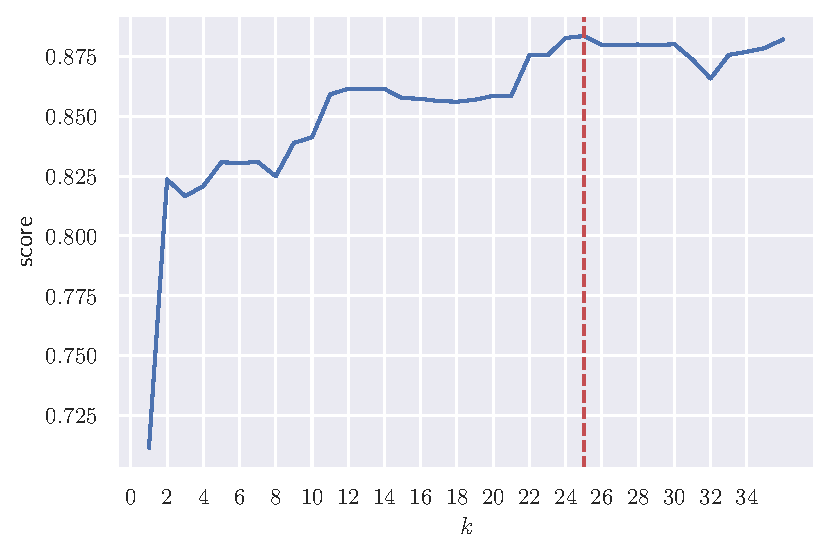
\includegraphics{kbest}
    \caption{Cross validation score for different $k$ values}%
    \label{fig:feature_cross}
\end{figure}

\begin{table}[H]
    \centering
    \caption{Table of the selected features (25)}%
    \label{tab:features}
    \begin{tabular}{lr}
\toprule
          Variable &     Score \\
\midrule
    koi\_steff\_err1 &  0.187327 \\
          koi\_prad &  0.183411 \\
    koi\_steff\_err2 &  0.172951 \\
     koi\_prad\_err1 &  0.159601 \\
 koi\_duration\_err2 &  0.157072 \\
 koi\_duration\_err1 &  0.155455 \\
     koi\_prad\_err2 &  0.153358 \\
     koi\_srad\_err1 &  0.137056 \\
     koi\_model\_snr &  0.135153 \\
        koi\_period &  0.128600 \\
  koi\_time0bk\_err1 &  0.125205 \\
  koi\_time0bk\_err2 &  0.124540 \\
    koi\_slogg\_err2 &  0.123757 \\
    koi\_slogg\_err1 &  0.119153 \\
         koi\_steff &  0.115552 \\
   koi\_period\_err2 &  0.110208 \\
   koi\_period\_err1 &  0.108851 \\
    koi\_insol\_err2 &  0.106811 \\
         koi\_depth &  0.106059 \\
    koi\_insol\_err1 &  0.105953 \\
           koi\_teq &  0.102837 \\
         koi\_insol &  0.101366 \\
        koi\_impact &  0.100266 \\
          koi\_srad &  0.099673 \\
\bottomrule
\end{tabular}

\end{table}